\chapter{Optimización económica}
\label{cap:optimizacion}

\section{Decidir es optimizar}

Toda la teoría de la empresa converge en una pregunta: \emph{¿cuánto producir para ganar lo más posible?} Optimizar es buscar el valor de una variable de decisión —la cantidad, el precio, la combinación de productos— que hace máxima (o mínima) una función objetivo. Con el cálculo del Capítulo~\ref{cap:marginal} ya tenemos la llave: en un máximo «liso», la pendiente de la función objetivo es cero \cite{chiang}.

\section{Optimización libre: el máximo beneficio}

Queremos maximizar el beneficio $\Pi(q) = I(q) - C(q)$. El procedimiento tiene dos pasos.

\paragraph{Condición de primer orden (CPO).} En el óptimo, la derivada se anula:
\begin{equation}
\Pi'(q^{*}) = 0 \;\Longleftrightarrow\; I'(q^{*}) = C'(q^{*}) \;\Longleftrightarrow\; \boxed{\img = \cmg}.
\label{eq:cpo}
\end{equation}
Reencontramos, ahora con todo rigor, la regla anticipada en capítulos anteriores: \textbf{se produce hasta que el ingreso marginal iguala al costo marginal}. La intuición es imbatible: mientras $\img > \cmg$, cada unidad extra agrega beneficio; cuando $\img < \cmg$, resta. El punto de quiebre es el óptimo.

\paragraph{Condición de segundo orden (CSO).} La CPO también la cumpliría un \emph{mínimo}. Para asegurar que es un máximo, la función debe ser cóncava ahí: la segunda derivada negativa,
\begin{equation}
\Pi''(q^{*}) < 0.
\label{eq:cso}
\end{equation}

\begin{ejemplo}[El beneficio máximo del kiosco]
Retomemos $\Pi(q) = -\tfrac12 q^2 + 50q - 50$ del Capítulo~\ref{cap:funciones}. La CPO:
\[
\Pi'(q) = -q + 50 = 0 \;\Longrightarrow\; q^{*} = 50.
\]
La CSO: $\Pi''(q) = -1 < 0$, así que es efectivamente un máximo. El beneficio óptimo es
\[
\Pi(50) = -\tfrac12(2500) + 50(50) - 50 = -1250 + 2500 - 50 = 1200.
\]
Producir 50 unidades diarias maximiza el beneficio en \$1200. Ni una más (empezaría a perder en el margen), ni una menos (dejaría ganancia sobre la mesa).
\end{ejemplo}

\begin{figure}[htbp]
\centering
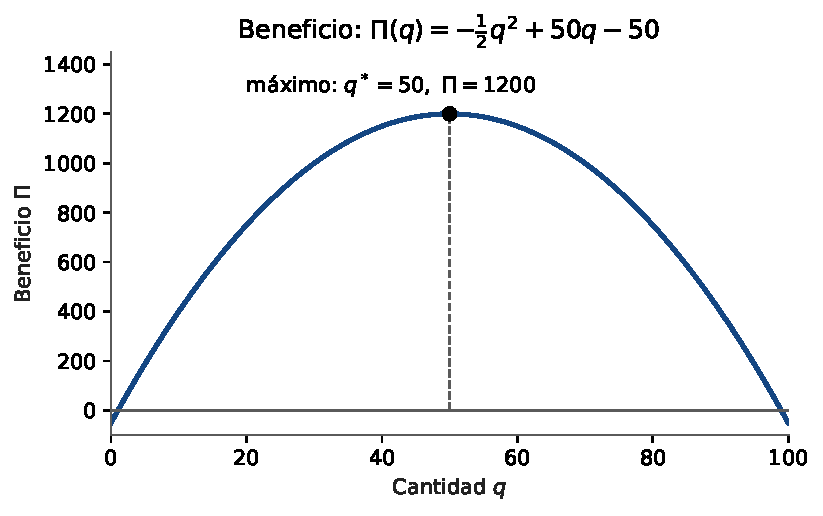
\includegraphics[width=0.72\linewidth]{figuras/beneficio}
\caption{La función de beneficio es una parábola cóncava: su vértice (donde la pendiente es cero, $\Pi'=0$) marca la cantidad que maximiza la ganancia.}
\label{fig:beneficio}
\end{figure}

\section{Optimización con restricciones: cuando los recursos son escasos}

En la gestión real rara vez se decide una sola cantidad sin límites. Lo habitual es elegir \emph{cuánto producir de varios productos} con \textbf{recursos limitados}: horas de máquina, presupuesto, materia prima. Esto es un problema de \emph{optimización con restricciones}, y cuando tanto el objetivo como las restricciones son lineales, se llama \textbf{programación lineal}.

Su forma general: elegir cantidades $x_1,\dots,x_n$ que
\begin{equation}
\max\ \ Z = \sum_{j} c_j x_j
\qquad\text{sujeto a}\qquad
\sum_{j} a_{ij}\,x_j \le b_i,\quad x_j \ge 0,
\end{equation}
donde $c_j$ es el margen de cada producto, $a_{ij}$ cuánto recurso $i$ consume el producto $j$, y $b_i$ la disponibilidad del recurso $i$. La solución óptima siempre se encuentra en un \emph{vértice} de la región factible —el polígono de combinaciones que respetan todas las restricciones—, resultado central de la teoría de la programación lineal.

\begin{ejemplo}[Mezcla de producción]
Una fábrica produce sillas ($x_1$, margen \$40) y mesas ($x_2$, margen \$60). Cada silla usa 2~h de carpintería y cada mesa 4~h; hay 100~h disponibles. Además se dispone de 80~h de pintura, con 1~h por silla y 1~h por mesa. El problema es
\[
\max\ \ 40x_1 + 60x_2 \quad\text{s.a.}\quad 2x_1+4x_2\le 100,\ \ x_1+x_2\le 80,\ \ x_1,x_2\ge 0.
\]
La solución óptima asigna las horas escasas al producto que más margen aporta por hora de recurso. Resolverlo a mano con dos productos es viable; con decenas de productos y restricciones se vuelve imposible, y por eso recurrimos a la computadora.
\end{ejemplo}

\begin{labbox}
Dos herramientas, según el problema. Para la \emph{optimización libre} (máximo beneficio), el laboratorio usa \texttt{sympy}: derivar el beneficio y resolver $\Pi'(q)=0$ con \texttt{sympy.solve(sympy.diff(I-C, q), q)}, verificando el signo de la segunda derivada. Para la \emph{optimización con restricciones}, se usa \texttt{PuLP}: se declaran las variables, la función objetivo y las restricciones casi con las mismas palabras de la formulación matemática, y el \emph{solver} encuentra el vértice óptimo. La fórmula~\eqref{eq:cpo} y el método de \texttt{PuLP} son las dos caras —cálculo y álgebra lineal— de la misma idea de optimizar.
\end{labbox}

\begin{ideabox}
\textbf{Por qué importa.} La optimización es el punto donde la economía deja de describir y empieza a \emph{recomendar}: dado un objetivo y unas restricciones, dice cuál es la mejor decisión posible. Es el corazón cuantitativo de la gestión.
\end{ideabox}

\section{Síntesis del capítulo}

Maximizar el beneficio lleva a la regla $\img=\cmg$ (CPO), validada por la concavidad (CSO). Cuando hay recursos escasos y varios productos, la programación lineal generaliza el problema. En el próximo capítulo aplicamos la optimización a un escenario estratégico: dos empresas que compiten y deben anticipar la decisión de la rival.
